Para representar el \'arbol del segment tree vamos a utilizar un arreglo \texttt{T}. El resultado del nodo ra\'iz se guarda en \texttt{T[1]}. En general, si el resultado de un nodo se guarda en la posici\'on $p$, entonces el resultado de su hijo izquierdo se guarda en la posici\'on $2 \cdot p$ y el resultado de su hijo derecho se guarda en $2 \cdot p + 1$. Esta representaci\'on es v\'alida para cualquier \'arbol binario. De esta forma podemos guardar el segment tree construido para un arreglo \texttt{A} de largo $n$ en un arreglo \texttt{T} de largo a lo m\'as $4n$. 

El segment tree para el arreglo original quedar\'ia guardado en el arreglo de la siguiente forma:

\begin{minipage}{\columnwidth}
    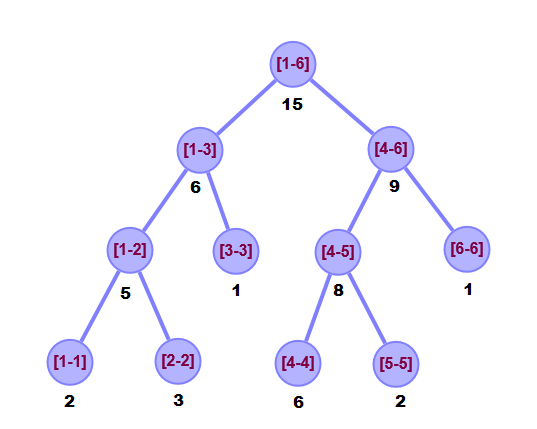
\includegraphics[width=\linewidth]{imag/segment_tree_suma}
    \label{example_st_casos}
\end{minipage}

\noindent \begin{minipage}{\linewidth}
    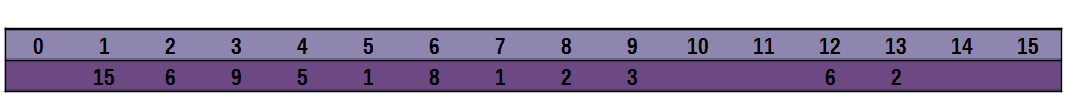
\includegraphics[width=\linewidth]{imag/arreglo2}
    \label{example_st_casos}
\end{minipage}

Creamos una clase \texttt{SegmentTree} que tiene como atributos al largo del arreglo \texttt{n}, al arreglo dado \texttt{A}, y al arreglo \texttt{T}, donde guardaremos los valores del \'arbol. El constructor de la clase inicializa los valores de los atributos y llama a la funci\'on \texttt{build()}.

\raggedbottom\lstinputlisting[style=java]{segment_tree_code/constructor.java}

El m\'etodo \texttt{build()} construye el segment tree. Recibe como par\'ametros \texttt{l} y \texttt{r}, que son los los extremos del rango del nodo y \texttt{nod} que es la posici\'on del nodo actual en el arreglo \texttt{T}. Inicialmente se llama a las funciones con \texttt{l = 1}, \texttt{r = n} y \texttt{nod = 1}, que son los valores correspondientes al v\'ertice ra\'iz.
  
Si el nodo actual es un nodo hoja (o sea, si \texttt{l == r}) entonces inicializamos el valor del nodo con el valor correspondiente del elemento del arreglo, que es \texttt{A[l]}.

Si no es as\'i preguntamos recursivamente los valores de los hijos y cuando estos sean respondidos, los combinamos y los guardamos como el valor del nodo.

Observe que en todos los m\'etodos calculamos el valor de \texttt{m} y llamamos a los hijos izquierdo y derecho con sus par\'ametros para \texttt{l}, \texttt{r} y \texttt{nod} correspondientes: \texttt{(l, m, 2*nod)} para el hijo izquierdo y \texttt{(m+1, r, 2*nod+1)} para el derecho.
\raggedbottom\lstinputlisting[style=java]{segment_tree_code/build.java}

El siguente m\'etodo es \texttt{query()}, correspondiente a la consulta en rango. Su versi\'on p\'ublica llama al m\'etodo privado. El privado recibe como argumentos a los extremos del rango de la consulta \texttt{a} y \texttt{b} adem\'as de los par\'ametros \texttt{l}, \texttt{r} y \texttt{nod}. Los primeros dos bloques \texttt{if} corresponden a los dos primeros casos del m\'etodo. Si el nodo no corresponde a ninguno de ellos, entonces preguntamos recursivamente a sus hijos, haciendo las llamadas con los par\'ametros correspondientes.

\raggedbottom\lstinputlisting[style=java]{segment_tree_code/query.java}

Por \'ultimo vamos a hablar del m\'etodo \texttt{update()} que lleva a cabo las actualizaciones de posici\'on. Este m\'etodo tiene tambi\'en su versi\'on p\'ublica.

Los primeros dos bloques \texttt{if} corresponden a los dos primeros casos del m\'etodo. Si el nodo no corresponde a ninguno de ellos, entonces preguntamos recursivamente a sus hijos, haciendo las llamadas con los par\'ametros correspondientes. Luego combinamos las respuestas, actualizamos los valores en el \'arbol y por \'ultimo retornamos el valor obtenido.


\raggedbottom\lstinputlisting[style=java]{segment_tree_code/update.java}